\section{Introducción}

Aunque las redes Narrowband IoT han habilitado despliegues masivos de sensores en entornos remotos, su seguridad descansa todavía sobre cimientos frágiles cuando se proyecta hacia el horizonte cuántico. 

\subsection{1.1 Motivación y Problema de Investigación}

Resulta particularmente llamativo observar cómo los protocolos de seguridad actuales en NB-IoT, diseñados bajo supuestos de computación clásica, enfrentan una obsolescencia silenciosa pero acelerada. Dispositivos desplegados en exploración profunda --monitoreo oceánico, minería subterránea o vigilancia ambiental en zonas inhóspitas-- transmiten datos que pueden conservar valor crítico durante décadas. Sin embargo, la amenaza ``harvest-now-decrypt-later'' convierte esas transmisiones en activos vulnerables desde el momento mismo de su captura.

La computación cuántica, mediante algoritmos como el de Shor, desmantela con eficiencia polinomial los fundamentos de RSA y ECC, mientras que Grover reduce a la mitad la seguridad efectiva de esquemas simétricos. En entornos NB-IoT, donde el consumo energético y el ancho de banda son extremadamente limitados, estas vulnerabilidades no representan meras hipótesis teóricas. Representan un riesgo operativo concreto.

Estudios recientes destacan que muchas implementaciones IoT actuales exhiben brechas significativas al considerar optimizaciones para dispositivos restringidos \cite{Liu2024_PQC_IoT}. Lejos de ser un problema marginal, la convergencia entre restricciones de hardware NB-IoT y la escalada de capacidades cuánticas configura uno de los desafíos más urgentes en ciberseguridad industrial.

\begin{table}[t]
\centering
\caption{Comparación entre Amenazas Clásicas y Cuánticas en NB-IoT}
\label{tab:amenazas}
\begin{tabular}{|l|l|l|}
\hline
\textbf{Aspecto} & \textbf{Amenaza Clásica} & \textbf{Amenaza Cuántica} \\
\hline
Criptografía afectada & Ataques de fuerza bruta, side-channel & Shor (clave pública), Grover (simétrica) \\
\hline
Tiempo de ruptura & Años/décadas & Horas/días (con QC escalable) \\
\hline
Impacto en datos históricos & Limitado & Alto (harvest-now-decrypt-later) \\
\hline
Requisitos de mitigación & Actualizaciones periódicas & Migración completa a PQC \\
\hline
\end{tabular}
\end{table}

\begin{figure}[t]
\centering
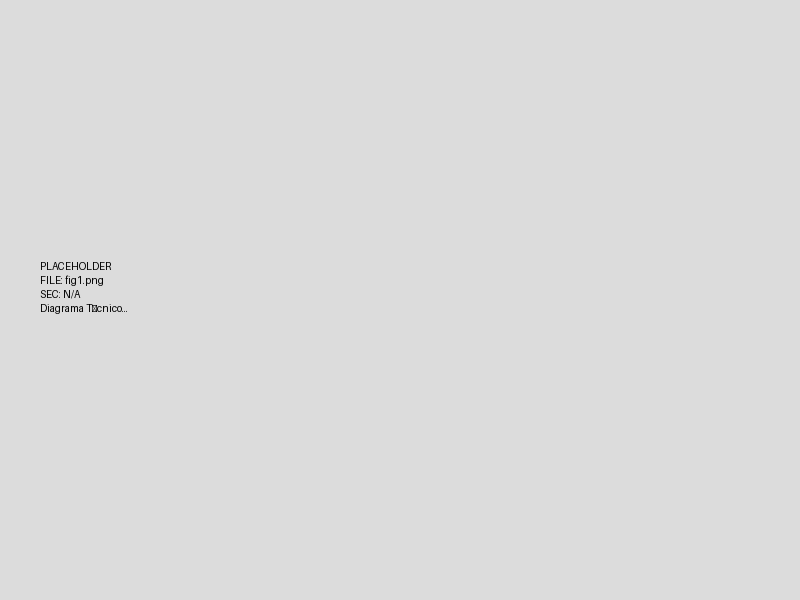
\includegraphics[width=\linewidth]{fig1.png}
\caption{Arquitectura típica de NB-IoT mostrando capas de percepción, red de acceso y núcleo EPC junto con flujos de comunicación en escenarios de exploración profunda.}
\label{fig:arquitectura_nb_iot}
\end{figure}

\subsection{1.2 Contribuciones Principales}

Particularmente revelador es el hecho de que pocas propuestas hasta la fecha logran equilibrar resistencia cuántica con las severas restricciones operativas de NB-IoT en campo. Este trabajo aborda precisamente esa brecha.

Las contribuciones centrales incluyen: primero, un análisis detallado de vectores de amenaza específicos en comunicaciones de exploración profunda; segundo, el diseño de una arquitectura híbrida que integra onboarding post-cuántico en el plano de control con protección ligera en el plano de datos; tercero, una evaluación cuantitativa de métricas críticas --latencia, consumo energético y overhead de comunicación-- bajo condiciones realistas.

A diferencia de enfoques genéricos, la propuesta mantiene compatibilidad con estándares 3GPP mientras incorpora primitivas PQC optimizadas. Investigaciones previas en criptografía resistente basada en lattices para IoT \cite{Althobaiti2021_QuantumResistant} sirven como base sólida, aunque requieren adaptaciones sustanciales para los escenarios de despliegue remoto que motivan este estudio.

\subsection{1.3 Estructura del Artículo}

El resto del documento se organiza de manera que facilite tanto la comprensión conceptual como la reproducción técnica. La Sección 2 revisa antecedentes y estado del arte. La Sección 3 profundiza en las amenazas específicas de exploración profunda. Posteriormente, la Sección 4 presenta la arquitectura propuesta, seguida de la metodología de implementación y evaluación en la Sección 5. Los resultados y análisis ocupan la Sección 6, mientras que la discusión de implicaciones aparece en la Sección 7. Finalmente, las conclusiones y líneas de trabajo futuro cierran el artículo.